\documentclass{article}
\usepackage{graphicx} % Required for inserting images
\usepackage{kotex}
\usepackage{minted} % 소스 코드 하이라이팅
\usemintedstyle{friendly}

\title{프로그래밍언어론 hw4}
\author{C011013 권찬}
\date{2024.05.30}

\begin{document}

\maketitle

\section{LISP}
\quad LISP는 LISt Processing language의 줄임말로, 대표적인 함수형 언어입니다.\\
포트라인에 이어 두번째로 오래된 고급 프로그래밍 언어이며, 모든 데이터를 연결 리스트로 처리합니다.\\
괄호의 활용도가 높은 것이 특징입니다.\\
명확한 표준이 존재하지 않아서 여러 파생 언어(방언)가 만들어졌는데, 이를 모아 표준화한 것이 Common LISP 입니다.\\\\
LISP를 구성하는 기초 단위는 atom, list, string 3가지 입니다.\\
연산, 함수 호출 등을 할 때는 전위 표기를 사용합니다.\\
예를 들어 3 + 4 를 한다면 LISP에서는 (+ 3 4) 와 같이 괄호 안에 전위 표현식을 작성합니다.\\
LISP에서는 데이터를 리스트의 구조로 표현하는데, 예를 들면 (A (B C) D (E (F G))) 와 같이 표현합니다.\\
이를 Figure~\ref{fig-1}과 같이 연결리스트로 나타낼 수 있습니다.

\begin{figure}[!htb]
    \centering
    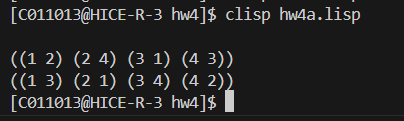
\includegraphics[width=0.5\linewidth]{hw4_img1.png}
    \caption{연결리스트로 나타낸 모습}
    \label{fig-1}
\end{figure}

\section{과제 코드 작동 방식}
\subsection{hw4a: N-Queen}
\subsubsection{알고리즘}

\quad N-Queen 문제를 풀기 위해, 먼저 생각할 수 있는 것은, 퀸은 하나의 가로줄에 하나만 존재해야 한다는 것을 쉽게 떠올릴 수 있습니다.\\
하나의 가로줄에 여러 퀸이 있으면 서로가 서소를 가로 방향으로 공격할 수 있기 때문입니다.\\
따라서 각각의 가로줄마다 퀸을 임의 세로줄에 하나씩 배치해보면서 지금 가로줄에서 이 세로줄 위치에 퀸을 배치했을 때 서로 공격할 수 있는지 체크하고, 만약 공격할 수 있다면 그 세로줄에는 배치할 수 없으므로 그 케이스는 건너 뛰고, 배치할 수 있다면 그 위치에 일단 배치한 후, 다음 가로줄로 넘어가 이어서 퀸을 배치해봅니다.\\
위와 같이 일단 모든 경우의 수를 시도해보다가 중간에 안되는 경우를 만났을 때 뒤로 돌아가는 알고리즘을 백트래킹이라고 하며, 재귀를 이용해 구현할 수 있습니다.\\
저는 아래와 같은 solve 함수를 작성하여 위에 설명한 알고리즘을 적용하였습니다.\\\\
\textbf{1. solve 함수}\\
\begin{minted}[frame=single, framesep=10pt, breaklines=true, fontsize=\small, linenos=true]{c}
(defun solve(line pos_list)
  (when (eql line 4) ; line == 4 이면
    (print pos_list)
    (return-from solve)
  )

  ; line < 4 이면,
  (loop for i from 1 to 4 do ; 다음 라인에 1, 2, 3, 4를 모두 배치해본다.
    (when (check (+ line 1) i pos_list) ; 다음 line에 i 위치가 퀸을 배치할 수 있는 위치라면
      (setq new_pos_list (append pos_list (list (list (+ line 1) i)) ) ) ; 퀸을 배치하고 재귀 호출
      (solve (+ line 1) new_pos_list)
    )
  )
)
\end{minted}
solve 함수는 몇 번째 line까지 잘 배치했는지를 나타내는 line, 그때까지 배치한 퀸의 좌표를 나타내는 pos\_list 를 매개변수로 받습니다.\\\\
현재 라인이 4번째 라인이라면 4번째 라인까지 퀸을 잘 배치했다는 뜻이므로 N = 4, N-Queen 문제를 해결한 케이스라는 것을 나타냅니다. 따라서 배치한 각 퀸의 좌표를 출력하고 재귀를 종료합니다.\\\\
만약 그 이전 라인이라면, 그 이전 line 번째 라인까지는 잘 배치했다는 의미이므로, 그 다음 라인에 대해 각각의 세로 위치(pos)를 확인하면서 그 위치에 퀸을 배치해도 문제가 없는지 check 함수를 사용해 확인합니다. (check함수는 뒤에 설명하겠습니다.) 이렇게 확인했을 때 문제가 없었다면 그 위치에 퀸을 배치하여 pos\_list에 추가해주고, line을 1 증가시킨 값과 새로운 pos\_line을 매개변수로 하여 solve 함수를 재귀적으로 호출합니다.\\\\
\textbf{2. check 함수}\\
\begin{minted}[frame=single, framesep=10pt, breaklines=true, fontsize=\small, linenos=true]{c}
; 각 배치할 때마다 상하좌우 대각선 체크 
(defun check(line pos pos_list)
  ; 가로줄에는 1개씩 배치하니까 체크할 필요가 없다.
  
  ; 세로줄에 겹치는 부분이 있는지 확인
  (loop for check_line from 1 to 4 do
    (when (eql check_line line)
      (return )
    )

    (loop for check_list in pos_list do
      (when (equal (list check_line pos) check_list) 
        (return-from check nil)
      )
    )
  )

  ; 우하 대각선에 겹치는 부분이 있는지 확인
  (loop for i from 1 to 4 do
    (setq check_line (+ i line))
    (setq check_pos  (+ i pos))
    
    (when (or (> check_line 4) (> check_pos 4))
      (return )
    )

    (loop for check_list in pos_list do
      ;; (print (equal (list check_line check_pos) check_list) )
      (when (equal (list check_line check_pos) check_list) 
        (return-from check nil)
      )
    )
  )

  ; 좌상 대각선에 겹치는 부분이 있는지 확인
  (loop for i from 1 to 4 do
    (setq check_line (- line i))
    (setq check_pos  (- pos i))
    
    (when (or (< check_line 1) (< check_pos 1))
      (return )
    )

    (loop for check_list in pos_list do
      (when (equal (list check_line check_pos) check_list) 
        (return-from check nil)
      )
    )
  )

  ; 좌하 대각선에 겹치는 부분이 있는지 확인
  (loop for i from 1 to 4 do
    (setq check_line (+ i line))
    (setq check_pos  (- pos i))
    
    (when (or (> check_line 4) (< check_pos 1))
      (return )
    )

    (loop for check_list in pos_list do
      (when (equal (list check_line check_pos) check_list) 
        (return-from check nil)
      )
    )
  )

  ; 우상 대각선에 겹치는 부분이 있는지 확인
  (loop for i from 1 to 4 do
    (setq check_line (- line i))
    (setq check_pos  (+ i pos))
    
    (when (or (< check_line 1) (> check_pos 4))
      (return )
    )

    (loop for check_list in pos_list do
      (when (equal (list check_line check_pos) check_list) 
        (return-from check nil)
      )
    )
  )

  (return-from check T)
)
\end{minted}
\quad check함수는 line, pos, pos\_list 를 매개변수로 받습니다.\\
이 함수는 지금까지 퀸을 pos\_list에 들어있는 대로 배치했을 때 line, pos 위치에 추가적으로 퀸을 배치할 수 있으면 T를, 배치할 수 없다면 nil을 반환합니다.\\
LISP에서는 T 가 True를 의미하고, nil이 False를 의미하므로 check 함수의 반환값을 조건문으로 넘겨서 확인하면 원하는 위치에 퀸을 둘 수 있는지 없는지 확인할 수 있습니다.\\\\
퀸을 line, pos 위치에 배치할 수 있다는 말은 line, pos 위치에 퀸을 배치했을 때 그 주변 가로줄 (지금 알고리즘은 가로줄 하나에 퀸을 하나씩만 배치하므로 사실 확인할 필요가 없습니다.) 그 위치의 세로줄, 그 위치로부터 대각선 위치에 아무런 퀸도 없다는 뜻과 같습니다.\\\\
따라서 반복문을 돌면서 세로줄 위치를 확인하면서 해당 위치에서 퀸을 발견하면 즉시 nil을 반환하고, 그렇지 않으면 넘어가도록 코드를 작성하였습니다.\\
대각선의 경우, 임의 위치로부터 좌상, 우상, 좌하, 우하 4가지 경우를 각각 확인하여 퀸이 대각선 위치에 존재하는지 확인합니다.

\subsubsection{실행결과}
\begin{figure}[!htb]
    \centering
    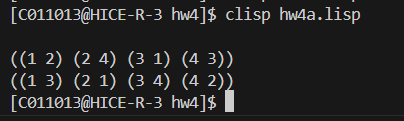
\includegraphics[width=0.5\linewidth]{hw4_img2.png}
    \caption{N-Queen 과제 코드 실행 결과}
    \label{fig-2}
\end{figure}

\subsection{hw4b: Insertion Sort}
\subsubsection{알고리즘}

\quad Insertion Sort 알고리즘은 첫번째 인덱스부터 점차 증가하도록 반복을 돌면서, 자신보다 작은 인덱스 위치에 있는 모든 값을 돌아보며 자신보다 크면 넘어가고 자신보다 작으면 그 위치에 자신을 끼워넣는 정렬 알고리즘입니다.\\
저는 아래와 같은 solve 함수를 작성하여 위에 설명한 알고리즘을 적용하였습니다.\\\\
\textbf{1. solve 함수}\\
\begin{minted}[frame=single, framesep=10pt, breaklines=true, fontsize=\small, linenos=true]{c}
(defun solve(key now_list)
  (when (>= key (length now_list)) ; 현재 보고 있는 인덱스 (key) 가 now_list 인덱스 범위를 벗어났다면 정렬이 완료된 것
    (princ (list "최종 결과"))
    (princ now_list)
    (print "")
    (return-from solve)
  )

  (when (eql key 1) ; key가 1번째 인덱스라면 인자로 넘어온 리스트는 정렬되지 않은 초기 정렬이므로 출력한다.
    (princ (list "시작 리스트"))
    (princ now_list)
    (print "")
  )

  (when (/= key 1) ; key가 1번째 인덱스도 아니고, now_list 범위 안에 있다면 정렬 중이므로 중간 과정을 출력한다.
    (princ (list (- key 1) " 단계"))
    (princ now_list)
    (print "")
  )
  
  (setq new_list (list )) ; 현재 단계에서 정렬한 중간 단계 리스트를 만들기 위해, 빈 리스트를 생성한다.
  (setq finish 0) ; 
  (loop for index from 0 to key do ; key 보다 작은 인덱스 범위를 돌면서 체크한다.
    (when (< (nth index now_list) (nth key now_list)) ; key 앞에 있는 원소와 key 위치 원소를 비교해서 key 위치 원소가 더 크면 앞의 원소를 그대로 중간 결과 리스트에 넣는다.
      (setq new_list (append new_list (list (nth index now_list)) ))
    )
    (when (>= (nth index now_list) (nth key now_list)) ; key 이전에 있는 원소와 key 원소를 비교했을 때 key가 크거나 같으면 이 위치에 key 원소를 끼워넣는다.
      (setq new_list (append new_list (list (nth key now_list)) )) ; 키를 먼저 넣고
      (setq finish index) ; 키 원소가 삽입된 위치, 이 위치 이후에 있는 배열 값들을 모두 중간 결과 리스트에 넣는다.
      (when (< index key)
        (setq new_list (append new_list (list (nth index now_list)) )) ; 키 뒤에 남아있는 배열 값들을 차례대로 새 리스트에 넣는다.
        (setq finish (+ 1 index))
      )
      (return )
    )
  )

  (loop for index from finish to (- (length now_list) 1) do
    (when (/= index key)
      (setq new_list (append new_list (list (nth index now_list)) )) ; 리스트 뒤에 있는 값들을 넣는다.
    )
  )

  (solve (+ key 1) new_list)
)
\end{minted}
solve 함수는 현재 몇 번째 인덱스를 기준으로 보고 있는지를 key로, 지금까지 정렬된 중간 결과 리스트를 now\_list로 하여 매개변수로 받습니다.\\\\
만약 현재 보고 있는 key가 배열의 크기 이상이라면, 인덱스 범위를 벗어났으므로 모든 정렬이 끝났음을 의미합니다.\\
따라서 현재 인자로 들어온 중간 결과 리스트를 결과 리스트로 출력하고 재귀를 종료합니다.\\\\
만약 key가 1이라면 인자로 넘어온 리스트는 정렬되지 않은 초기 정렬이므로 과제 조건에 따라 출력합니다.\\
만약 key가 1보다 큰 배열 범위 안이라면, 정렬하고 있는 중간 결과이므로, 과제 가점 조건에 따라 중간결과를 출력합니다.\\\\
현재 단계에서 넘어온 key 인덱스 원소를 기준으로, 그 이전 인덱스에 있는 모든 원소값들을 key가 가리키는 원소값과 비교해봅니다.\\
만약 중간에 자신보다 작은 원소를 만난다면 그 원소 직후에 key가 가리키는 원소를 끼워넣어주고, 현재 단계의 정렬을 마무리합니다.\\
이때 배열 중간에 key를 끼워넣는 것이 구현하기 복잡할 것 같다고 생각하여, 빈 리스트를 만들고 빈 리스트를 직접 채우는 방식으로 구현하였습니다.\\
이렇게 구현할 때는 0부터 key까지 반복문을 돌면서, key보다 작은 원소는 그대로 빈 리스트에 추가해주고, key보다 큰 원소를 만났다면 그 때 key를 리스트에 추가한 뒤, 그 이후부터는 아직 추가하지 않은 원소들을 기존 순서대로 쭉 추가해줍니다.\\
이를 위해 key보다 큰 원소를 만났다면 그 위치를 finish 변수에 저장하고, key에 의해 밀린 원소를 finish 변수를 이용하여 추가해줍니다.\\

코드에서 38번째 줄부터는 key 이후의 원소들을 그대로 리스트에 추가하여 중간 정렬된 리스트를 완성하고, key 값을 1 증가시키고, 완성된 중간 정렬 리스트를 인자로 하여 solve 함수를 재귀적으로 호출합니다.

\subsubsection{실행결과}
\begin{minted}[frame=single, framesep=10pt, breaklines=true, fontsize=\small, linenos=true]{c}
(print "TC 1")
(print "")
(solve 1 (list 11 33 23 45 13 25 8 135))
(print "TC 2")
(print "")
(solve 1 (list 83 72 65 54 47 33 29 11))
\end{minted}

위와 같이 2개 테스트케이스에 대해 코드를 실행하였습니다.
\begin{figure}[!htb]
    \centering
    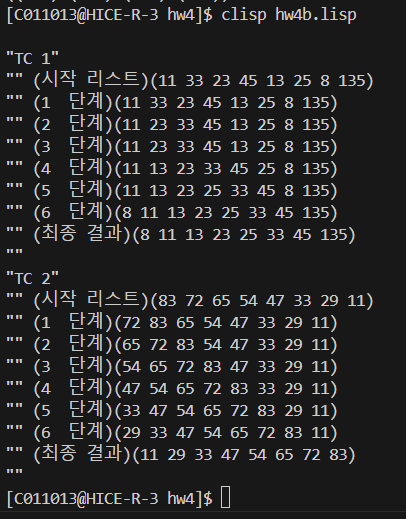
\includegraphics[width=0.5\linewidth]{hw4_img3.png}
    \caption{Insertion Sort 과제 코드 실행 결과}
    \label{fig-2}
\end{figure}

\section{어려웠던 점}
\quad 기존 명령형 언어가 아닌 함수형 언어로 코드를 작성하는 것이 어색했고, 무엇보다 중위 표기식을 항상 사용하다가 전위 표기식으로 수식을 작성하려고 하니 매우 헷갈렸습니다. 그래도 함수형 프로그래밍에 대해 경험해볼 수 있어서 매우 뜻깊은 과제였습니다.

\end{document}